%%%%%%%%%%%%%%%%%%%%%%%%%%%%%%%%%%%%%%%%%%%%%%%%%%%%%%%%%%%%%%%%%%%%%%%%%%%%%%%%
%2345678901234567890123456789012345678901234567890123456789012345678901234567890
%        1         2         3         4         5         6         7         8

\documentclass[letterpaper, 10 pt, conference]{ieeeconf}   % Comment this line out if you need a4paper

%\documentclass[a4paper, 10pt, conference]{ieeeconf}      % Use this line for a4 paper

\IEEEoverridecommandlockouts                              % This command is only needed if 
                                                          % you want to use the \thanks command

\overrideIEEEmargins                                      % Needed to meet printer requirements.

%In case you encounter the following error:
%Error 1010 The PDF file may be corrupt (unable to open PDF file) OR
%Error 1000 An error occurred while parsing a contents stream. Unable to analyze the PDF file.
%This is a known problem with pdfLaTeX conversion filter. The file cannot be opened with acrobat reader
%Please use one of the alternatives below to circumvent this error by uncommenting one or the other
%\pdfobjcompresslevel=0
%\pdfminorversion=4

% See the \addtolength command later in the file to balance the column lengths
% on the last page of the document

% The following packages can be found on http:\\www.ctan.org
\usepackage{graphicx} % for pdf, bitmapped graphics files
%\usepackage{epsfig} % for postscript graphics files
%\usepackage{mathptmx} % assumes new font selection scheme installed
%\usepackage{times} % assumes new font selection scheme installed
%\usepackage{amsmath} % assumes amsmath package installed
%\usepackage{amssymb}  % assumes amsmath package installed
\usepackage{algorithm, algorithmic}

\title{\LARGE \bf
Project I Report for COM S 4720 Spring 2025: Subtitle*
}


\author{Noah Miller}


\begin{document}



\maketitle
\thispagestyle{empty}
\pagestyle{empty}


%%%%%%%%%%%%%%%%%%%%%%%%%%%%%%%%%%%%%%%%%%%%%%%%%%%%%%%%%%%%%%%%%%%%%%%%%%%%%%%%
\begin{abstract}
	This paper will attempt to describe the searching algorithm written by the author in order to solve a path finding question in which the criteria used to define better algorithms are those that find the shortest path by number of steps, and the quickest algorithm to run.
	The finalized algorithm is an attempted implementation of A-star ~\cite{hart1968formal}. The method is created mostly from what was described in class, and what could be recalled at time of writing. The algorithm has room for improvement, but succeeds in most all cases.
\end{abstract}


%%%%%%%%%%%%%%%%%%%%%%%%%%%%%%%%%%%%%%%%%%%%%%%%%%%%%%%%%%%%%%%%%%%%%%%%%%%%%%%%
%\section{COM S 4/5720 INSTRUCTIONS}
%Unless noted otherwise (mostly in this section), please follow the rules set by the instructions in the following sections.
%
%The submitted project report should be a compiled typeset pdf file using this template. The pdf is at most 3 pages (including references).
%
%Please give clear, rigorous, and correct descriptions about your proposed algorithm. Please also make sure your description aligns with your code. Please include appropriate references, if applicable (e.g., A-star algorithm~\cite{hart1968formal}).
%
\section{INTRODUCTION}

Searching algorithms have been a question for computer scientists for a very long time. Searching algorithms are primarily used in attempts to solve mazes or to traverse trees, which can be thought of much the same. The criteria for a good searching algorithm is that which finds the optimal path, i.e. shortest path, and finds it quickly. Many undergraduate computer science students are required to learn and understand some of the most integral searching algorithms. These algorithms included Breadth First Search ~\cite{moore1959shortest}. This algorithm has been around since 1959, with A-star breaking ground in 1968 ~\cite{hart1968formal}. Breadth First Search and other algorithms like it do not look forward, taking into account the goal. This means that in order to find the optimal path and be guaranteed of it, one must search every single node. This is not optimal in the criteria of the problem. As such A-star uses the future cost of a branch to decide whether or not to take it ~\cite{hart1968formal}. This means A-star more commonly finds the optimal path, and finds it quickly. When designed as intended it can be proved to find the optimal path.

\section{Implementation}

\subsection{Pseudocode}
There are some assumptions in this algorithm. These assumptions are that all movement costs are positive and that the goal is reachable from the starting point. Without these assumptions, there is no guarantee that the algorithm will find the shortest path.
This algorithm states to take every point in the visited section that has moves to be made and check all moves to find the cheapest. The cheapest here is the cost of moving to that section plus an expected future cost. This cost is normally some kind of loss function, such as L2 or the distance equation, and allows A-star to utilize the future in determining the present move. The pseudocode as written does have some redundancy in it, leading to a very slow algorithm, but when implemented with optimizations it does perform up to speed.
\begin{algorithm}[H]
	\caption{Attempted Implementation}
	\begin{algorithmic}[1]
		\renewcommand{\algorithmicrequire}{\textbf{Input:}}
		\renewcommand{\algorithmicensure}{\textbf{Output:}}
		\REQUIRE grid, start, end
		\ENSURE  path
		\\ \textit{Initialization} :
		\STATE  visited = \{\}
		\STATE reached = FALSE
		\\ \textit{Main Loop}
		\WHILE {not reached}
		\STATE minCost = $\infty$
		\STATE move = a direction to move in
		\FORALL {point, $p$, in visited}
		\STATE directions = moves possible
		\FORALL {direction in directions}
		\STATE $p_{new} = p$ + direction
		\IF {$p_{new}$ in visited}
		\STATE continue
		\ENDIF
		\STATE g($p_{new}$) = cost to get to $p_{new}$
		\STATE h($p_{new}$) = distance to end from $p_{new}$
		\STATE f($p_{new}$) = g($p_{new}$) + h($p_{new}$)
		\IF{f($p_{new}$) $<$ minCost}
		\STATE minCost = f($p_{new}$)
		\STATE move = $p_{new}$
		\ENDIF
		\ENDFOR
		\ENDFOR
		\IF{move = end}
		\RETURN path = path taken to move
		\ENDIF
		\STATE visited.add(move: (cost, path), where cost is the cost to move, and the path is the path taken to the move and the move taken
		\ENDWHILE
		\RETURN path
	\end{algorithmic}
\end{algorithm}

Some of the non optimal section of the algorithm is in the repeated computation of the cost of each movement. There is also redundancy in rechecking each direction for each point every single loop. These both will be addressed in actual implementation, although as it will be touched on later in the discussion, it has lead to some confusion.



\subsection{Actual Implementation}

The actual implementation follows the psuedocode closely, diverging in some key ways, some of which are beneficial and some of which seem to introduce errors. That is not to say they do not find a correct path which will be discussed in the results. The first implementation choice is that for "visited" set, that is a hash set in which each point keeps track of the cost to it and the path taken to it. This is to give an ease of which to get both values and use them later in the algorithm. This does take up more space in the process, but keeps the speed up and the ease of accessing information needed very near. The other implementation choice is to keep track of the best move from each point. This stores every top move choice in another hash set. It does not store all moves sorted, but rather only the top move. This does save on space but reduces the effectiveness. This will be discussed further in the "Discussion" section.

\section{Results}

The implemented algorithm pulling from the concept of A-star is able to complete all examples. When running the "main.py" supplied for the project, each example passes. There is also the question of speed. For an average of 10 runs over the 100 tests, the a-star adjacent algorithm ran for 239836443.4 nanoseconds, whereas Depth First Search (dfs) provided by the professor took 330706057.3 seconds. That is not the full story though, as the path taken also matters.
\begin{figure}[thpb]
	\centering
	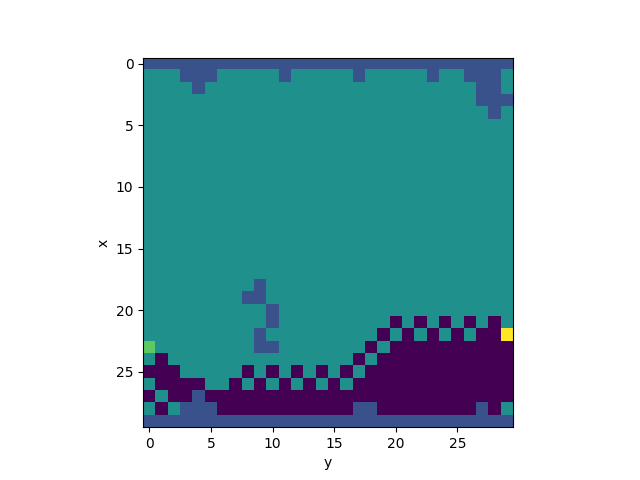
\includegraphics[scale=0.5]{ID5DFS.png}
	\caption{DFS ran on test example with ID: 5}
	\label{figurelabel}
\end{figure}
\begin{figure}[thpb]
	\centering
	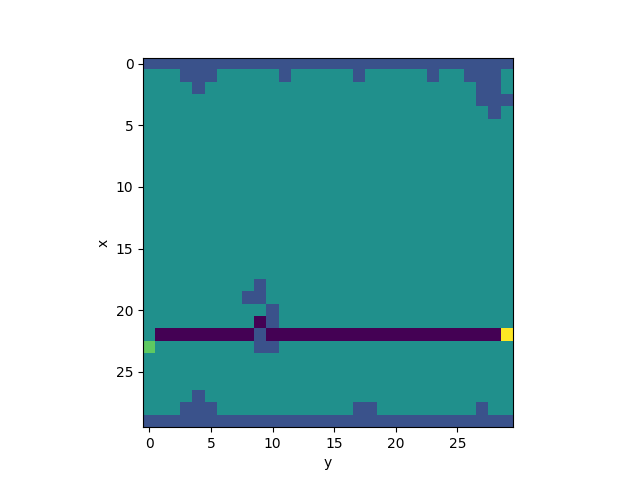
\includegraphics[scale=0.5]{ID5A.png}
	\caption{A-star ran on test example with ID: 5}
	\label{figurelabel}
\end{figure}
\begin{figure}[thpb]
	\centering
	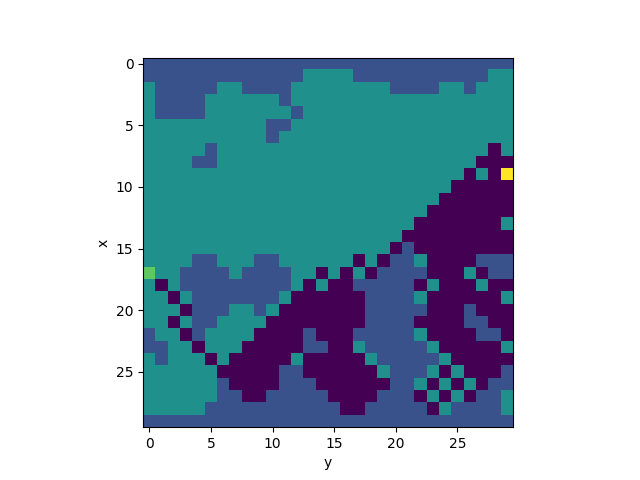
\includegraphics[scale=0.5]{ID10DFS.png}
	\caption{DFS ran on test example with ID: 10}
	\label{figurelabel}
\end{figure}
\begin{figure}[thpb]
	\centering
	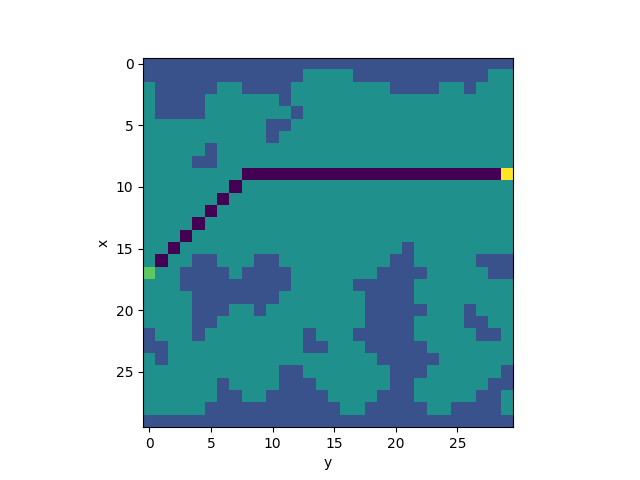
\includegraphics[scale=0.5]{ID10A.png}
	\caption{A-star ran on test example with ID: 10}
	\label{figurelabel}
\end{figure}
\begin{figure}[thpb]
	\centering
	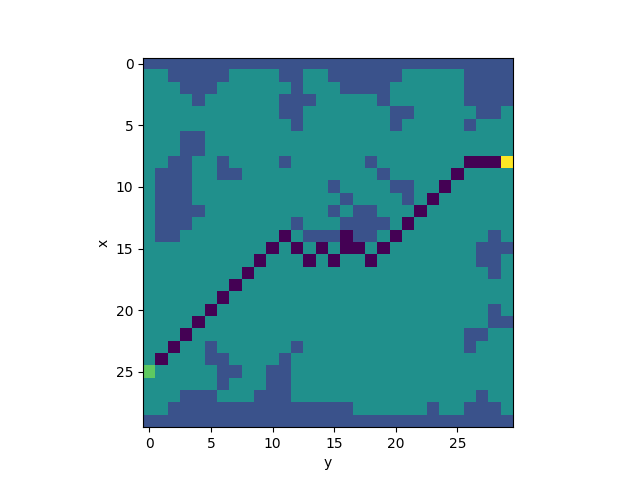
\includegraphics[scale=0.5]{FAILA.png}
	\caption{A-star ran on test example with ID: 24}
	\label{figurelabel}
\end{figure}

\section{Discussion}
As can be seen comparing Figures 1  3, to Figures 2 and 4, the A-star algorithm takes a much shorter path to the goal. This is not always the case though as Figure 5 shows. It is my contention that this is how best moves from each point is stored. As such the algorithm takes an extra step after finding itself near a boundary. There were many attempts to ramify the issue, but each resulted in much worse bugs such that the algorithm no longer finished each task. As can be seen from the results as well, the modified A-star algorithm operates at a similar speed to the dfs algorithm provided by the professor. This means that in the pursuit of the lowest cost path there is not a large tradeoff for speed.
\section{CONCLUSIONS}
This report explains an implementation of A-star used for finding the best path in a maze. The assumptions for each maze are such that each move takes a positive amount to move, and that each goal can be reached from the starting point. This implementation seems to perform much better than the provided algorithm from the professor, although does seem to have a flaw or two. Further implementation and work is needed to implement an optimal solution that is guranteed to find the optimal path. The algorithm still does find a better path than the naive implementation of dfs, but can be improved upon.
\addtolength{\textheight}{-12cm}   % This command serves to balance the column lengths
% on the last page of the document manually. It shortens
% the textheight of the last page by a suitable amount.
% This command does not take effect until the next page
% so it should come on the page before the last. Make
% sure that you do not shorten the textheight too much.

%%%%%%%%%%%%%%%%%%%%%%%%%%%%%%%%%%%%%%%%%%%%%%%%%%%%%%%%%%%%%%%%%%%%%%%%%%%%%%%%



%%%%%%%%%%%%%%%%%%%%%%%%%%%%%%%%%%%%%%%%%%%%%%%%%%%%%%%%%%%%%%%%%%%%%%%%%%%%%%%%



%%%%%%%%%%%%%%%%%%%%%%%%%%%%%%%%%%%%%%%%%%%%%%%%%%%%%%%%%%%%%%%%%%%%%%%%%%%%%%%%
\section*{ACKNOWLEDGMENT}

We would like to acknowledge Professor Wang, as without his work and teaching this report and implementation would not be possible.
%%%%%%%%%%%%%%%%%%%%%%%%%%%%%%%%%%%%%%%%%%%%%%%%%%%%%%%%%%%%%%%%%%%%%%%%%%%%%%%%


\bibliographystyle{IEEEtran}
\bibliography{bib}



\end{document}
